%------------------------------------------------------------------------------
% analysis.tex
%
% This illustrates the analysis of the proposed solution. 
%------------------------------------------------------------------------------
\chapter*{analisi della soluzione}
\addcontentsline{toc}{chapter}{Analisi della soluzione}
\label{analisi-della-soluzione}
In questa sezione del documento sono illustrate le scelte effettuate dallo studente durante la fase di progettazione in merito alle problematiche esposte nel precedente capitolo.

\section*{tipologia del simulatore}
\addcontentsline{toc}{section}{Tipologia del simulatore}
\label{analisi-della-soluzione-tipologia-del-simulatore}
Al fine di poter stabilire quale fosse la miglior tipologia di simulazione da adottare per lo specifico problema in questione, si sono studiati gli eventi di interesse per il sistema.

Data la necessità di conoscere lo stato attuale dei viaggi dei singoli mezzi e dello stato delle persone che vivono nella città, utilizzando una simulazione a tempo continuo è necessario calcolare molti più stati di quelli effettivamente utili avendo cosi uno spreco non indifferente della risorsa CPU. Inoltre, dato il requisito di distribuzione del sistema, si ha anche uno spreco non indifferente della risorsa rete per la comunicazione tra le parti di eventi non rilevanti.

Per i motivi appena citati, la scelta è ricaduta sulla realizzazione di una simulazione discreta a tempo reale, assicurandosi che l'architettura del sistema rispetti i vincoli e le invarianti tra eventi successivi.

\section*{gestione del tempo}
\addcontentsline{toc}{section}{Gestione del tempo}
\label{analisi-della-soluzione-gestione-del-tempo}
Il problema dell'utilizzo di valori temporali provenienti da un \english{clock} è intrinseco nel modo in cui tali valori sono reperiti.

Non esiste infatti modo di avere una risposta immediata alla richiesta di lettura (l'istante in cui si riceve il dato temporale è \keyword{sicuramente} successivo all'istante in cui è stata effettuata la richiesta di lettura) e non si può nemmeno compensare la latenza di lettura dato il \english{jitter} causato dallo \english{scheduler} (letture consecutive del valore temporale sono necessariamente accodate).

Diventa perciò evidente che l'unica strada percorribile è l'utilizzo di un \english{tempo relativo} che supporti però la coerenza con il tempo reale.

Dato che il sistema prevede l'interazione con l'utente, il rapporto tra tempo relativo e tempo reale è unitario; in particolare ogni \english{task} ha un tempo proprio, e tutte le comunicazioni di eventi si basano su intervalli temporali calcolati matematicamente a partire dall'intervallo precedente. Cosi facendo i tempi comunicati saranno sempre \english{offset} di uno zero logico (definito come il momento in cui la simulazione ha avuto inizio).

\section*{rappresentazione delle componenti}
\addcontentsline{toc}{section}{Rappresentazione delle componenti}
\label{analisi-della-soluzione-rappresentazione-delle-componenti}
Al fine di ottemperare alle caratteristiche esposte nel capitolo precedente, la città è stata suddivisa in quartieri (o distretti), i quali sono a loro volta costituiti da un insieme di incroci rappresentanti i punti d'intersezione delle strade che li compongono. Tale realtà è stata modellata secondo il modello ad attori che rende possibile la gestione dell'interazione tra le componenti del sistema e permette la gestione della concorrenza.

Data la particolarità del modello ad attori di poter delegare ad attori a lui dipendenti attività specifiche, l'intero sistema può essere pensato come ad una gerarchia di attori, cosi strutturata:

\begin{itemize}
\item{l'attore \keyword{città} ha il compito di fare da mediatore delle comunicazioni tra i diversi distretti che lo compongono;}
\item{l'attore \keyword{distretto} ha il compito di fare da mediatore delle comunicazioni tra i diversi incroci che lo compongono e l'attore città;}
\item{l'attore \keyword{incrocio} è la componente vera e propria che anima la simulazione.}
\end{itemize}

L'attore incrocio delega le attività alla base della simulazione, quali:

\begin{itemize}
\item{ricerca di una \english{route} per raggiungere una destinazione;}
\item{emulare le mansioni svolte dalle persone quando giungono a casa o al lavoro;}
\item{emulare il viaggio di un veicolo;}
\end{itemize}

ad altrettanti attori da lui gestiti direttamente. Attraverso questa scelta l'attore incrocio si rende cosi disponibile alla gestione di molteplici veicoli e/o persone senza rimanere impegnato in attività temporalmente onerose che rallenterebbero la simulazione facendole perdere l'effetto \keyword{tempo reale}.

\subsection*{gestione dei nomi}
\addcontentsline{toc}{subsection}{Gestione dei nomi}
\label{analisi-della-soluzione-gestione-dei-nomi}
La convenzione di nomenclatura adottata è una versione semplificata di quella utilizzata dal servizio \ac{dns}. Ogni incrocio facente parte della città ha un nome composto secondo la seguente convenzione:

\begin{center}
\textsc{nome\-città.nome\-distretto.nome\-incrocio}
\end{center}

La precedente convenzione impone una gerarchia nelle componenti facenti parte della città, rendendo perciò più semplice:

\begin{itemize}
\item{l'identificazione di un incrocio;}
\item{un eventuale estensione della struttura cittadina;}
\item{la verifica della correttezza della città implementata.}
\end{itemize}

\section*{ricerca di un percorso}
\addcontentsline{toc}{section}{Ricerca di un percorso}
\label{analisi-della-soluzione-ricerca-di-un-percorso}
Dopo quanto esposto nel precedente capitolo in merito alla ricerca di un percorso, si è deciso di adottare la tecnica delle \keyword{\english{route} dinamiche}.

L'adozione di questa tecnica impone l'implementazione di un algoritmo di \english{routing} che funga da ``navigatore'' per i veicoli che necessitino di determinare una strada che li conduca a destinazione.

Osservando la città da una diversa prospettiva, è possibile paragonarla ad un insieme di incroci che interconnessi tra loro formano una \keyword{rete \english{Ad-Hoc}}. Si è quindi cercato, un algoritmo in grado di risolvere il problema, nel campo delle reti \english{wireless}.

Dopo uno studio condotto per il corso di reti \english{Wireless}\footnote{di cui in allegato è reperibile il \english{paper} associato} si è osservato che l'algoritmo più adatto risulta essere \ac{aodv}, in quanto è risultato essere quello a \english{performance} migliori nel caso di reti statiche (ovvero reti in cui la posizione geografica dei nodi cambia di rado oppure mai). Si è perciò deciso di implementarne una versione semplificata all'interno del simulatore.

\section*{concorrenza}
\addcontentsline{toc}{section}{Concorrenza}
\label{analisi-della-soluzione-concorrenza}
Il sistema è implementato seguendo il paradigma del modello ad attori per la gestione della concorrenza e delle problematiche ad essa collegate. 

Similmente a quanto accade nel modello orientato agli oggetti, la filosofia alla base del modello ad attori è ``\english{everything is an actor}''. La differenza sostanziale con il modello ``orientato agli oggetti'' consiste nel fatto che mentre quest'ultimo prevede un'esecuzione tipicamente sequenziale, il modello ad attori è invece \keyword{intrinsecamente concorrente}.

Un attore è un'entità autonoma la quale opera in modo concorrente rispetto agli altri attori del sistema ed in modo del tutto asincrono, quindi non è necessaria sincronizzazione durante azioni di dialogo tra di loro. Ognuno di essi è definito da una coppia di elementi che lo contraddistinguono:

\begin{itemize}
\item{un nome univoco}
\item{un proprio \english{behavior} (in termini computazionali)}
\end{itemize}

Ogni attore, quando inattivo, si trova in particolare stato, denominato \keyword{idle} (stato in cui esso è in attesa di nuovi messaggi). Quando un messaggio è pendente nella \english{mailbox} dell'attore, quest'ultimo, accettandolo, ritorna ad essere attivo ed esegue una computazione dipendente da quanto specificato nel proprio \english{behavior}. Il risultato della computazione viene ``comunicato'' al sistema mediante l'esecuzione di una delle seguenti azioni:

\begin{itemize}
\item{invio di un messaggio ad un diverso attore;}
\item{creazione di un nuovo attore;}
\item{aggiornamento dello stato interno dell'attore stesso.}
\end{itemize}

\begin{figure}[h!]
\centering
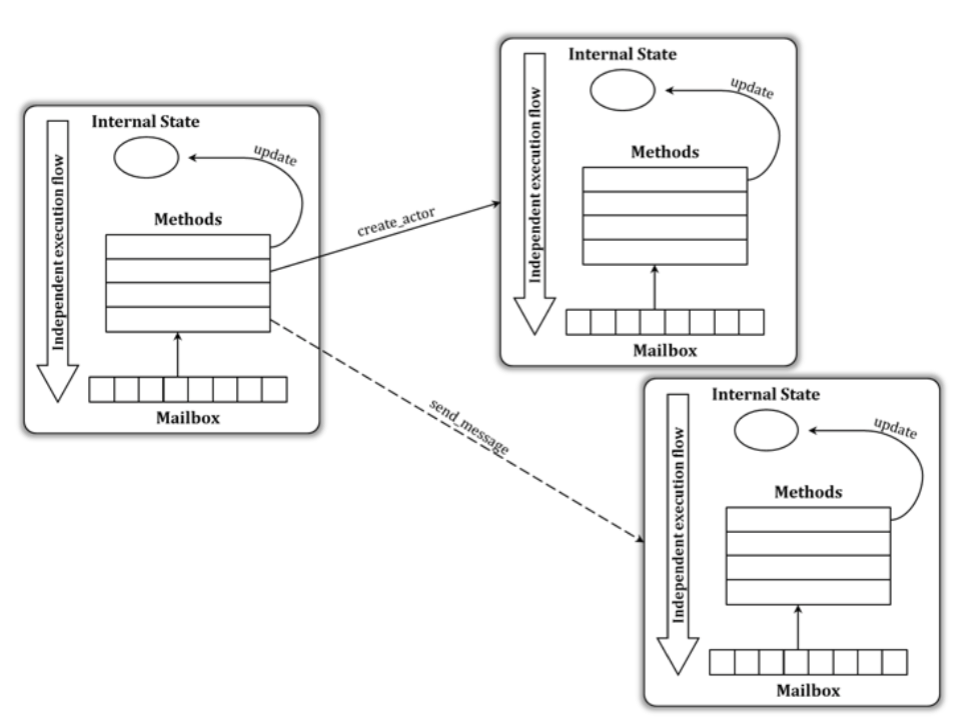
\includegraphics[scale=0.4]{images/analysis/Actor-model.png}
%\captionsetup{labelformat=empty}
\caption{Rappresentazione semplificata del modello ad attori}
\label{analisi-della-concorrenza-concorrenza-image-actor-model}
\end{figure}

La Figura \ref{analisi-della-concorrenza-concorrenza-image-actor-model} riassume quanto descritto circa la definizione del modello. E' possibile osservare gli elementi principali che lo costituiscono tra cui:

\begin{itemize}
\item{un proprio flusso di esecuzione indipendente dagli altri presenti;}
\item{le operazioni che esso può svolgere sul sistema come risultato dell'esecuzione di una particolare operazione.}
\end{itemize}

A conclusione della definizione del concetto di attore, è importante sottolineare che un attore \keyword{non condivide} con altri attori nel sistema il proprio stato interno, quindi per effettuare una modifica oppure ottenere informazioni in merito a tale stato è necessario inviare un esplicito messaggio all'attore interessato. E' opportuno inoltre specificare che l'ordine di arrivo dei messaggi, all'interno della \english{mailbox} di un attore, è del tutto indeterminato  a causa dell'asincronismo con cui essi sono inviati.

\subsection*{proprietà semantiche del modello}
\addcontentsline{toc}{subsection}{Proprietà semantiche del modello}
\label{analisi-della-concorrenza-concorrenza-proprietà-semantiche-del-modello}
Le proprietà semantiche chiave del modello ad attori sono:

\begin{itemize}
\item{incapsulamento dello stato interno;}
\item{atomicità d'esecuzione di ogni metodo come risposta ad un messaggio;}
\item{equità (\english{fairness}) nella gestione dell'avanzamento della computazione degli attori del sistema e nella consegna dei messaggi;}
\item{\english{location transparency}.}
\end{itemize}

\subsubsection*{incapsulamento}
La proprietà di incapsulamento (\english{encapsulation}) racchiude in sé quanto precedentemente detto nella definizione del concetto di attore circa il suo stato interno. Tale proprietà impone che due o più attori non possano condividere tra loro il proprio stato interno durante tutta l'esecuzione.

Volendo modificare o leggere lo stato interno di un attore, è necessario inviargli un esplicito messaggio ed attendere da lui una esplicita risposta.

Poiché il modello attori è intrinsecamente concorrente, è possibile che un messaggio giunga nella \english{mailbox} di un attore mentre quest'ultimo è impegnato nel processare un diverso messaggio giunto precedentemente nella \english{mailbox}\footnote{caso comune in caso di intensa attività}. Se per ipotesi fosse consentito, al secondo messaggio, di interrompere la gestione del primo per procedere all'immediata gestione del nuovo arrivato allora si otterrebbe come conseguenza che nel modello attori non sarebbe più possibile assumere che il comportamento di un attore, a fronte di un messaggio ricevuto, possa essere predeterminato in funzione del valore assunto dallo stato interno al momento della ricezione dello stesso.

\subsubsection*{atomicità}
La proprietà di atomicità (\english{atomicity}) evita la potenziale inconsistenza dello stato interno che si otterrebbe nel caso l'ipotesi effettuata nella sezione precedente circa l'eventuale assegnazione di livelli di priorità ai vari messaggi fosse verificata.

Nel modello ad attori, infatti, si impone che ciascun attore processi ogni messaggio in una unità atomica formata da tutte e sole le azioni necessarie atte a fornire una risposta al messaggio.

In tal modo si ottiene quindi una coda di esecuzione determinata dal momento di arrivo dei messaggi che permette di predeterminare il comportamento dell'attore a fronte dell'ordine di arrivo dei messaggi.

\subsubsection*{fairness}
La proprietà di \english{Fairness}\footnote{traducibile come ``equità e garanzia di esecuzione''} impone che ad ogni attore sia garantita la possibilità di computare se esso possiede almeno un messaggio a cui rispondere nella \english{mailbox}.

Impone inoltre che ogni messaggio inviato debba essere sempre consegnato all'attore destinatario con l'unica eccezione per quei messaggi destinati ad attori permanentemente o temporaneamente disabilitati nel sistema (attori impegnati in \english{loop} infiniti, che stanno tentando di eseguire un'operazione illecita oppure sono interdetti dalla ricezione di messaggi).

\subsubsection*{location transparency}
L'ultima proprietà semantica posseduta dal modello ad attori è la \english{location transparency}, ovvero la trasparenza rispetto alla dislocazione degli attori all'interno del sistema. 

Tale proprietà assicura l'importante caratteristica che consente ad un attore di non dipendere dalla posizione fisica all'interno del sistema. In questo modo un attore è in grado di scambiare messaggi con altri attori senza che esso sia a conoscenza del fatto che l'attore si trovi all'interno della stessa CPU o su un diverso computer collegato in rete dovendo di conseguenza impiegare tecniche di comunicazione differenti. Inoltre, mediante il rispetto di tale caratteristica, si ha la possibilità di effettuare una riconfigurazione del sistema in modo del tutto trasparente dalla logica di funzionamento.

L'indipendenza tra la locazione fisica e la locazione logica di ogni attore nel sistema, favorisce in tal senso un agile realizzazione di applicazioni distribuite.

\subsection*{stalli}
\addcontentsline{toc}{subsection}{Stalli}
\label{analisi-della-soluzione-concorrenza-stalli}
Dopo quanto illustrato sul modello ad attori è possibile notare come le uniche situazioni di stallo possibili si avrebbero solamente durante la fase di dialogo tra attori. Stallo possibile  in quanto ogni uno di essi possiede un unica risorsa \english{mailbox} la quale deve essere acceduta tramite mutua esclusione al fine di preservarne lo stato interno.

Al fine di evitare lo stallo si è deciso di invalidare la regola di Havender che sancisce l'accumulo di risorse, evitando quindi che un attore detenga l'accesso esclusivo a tali struttura dati quando debba comunicare con più attori.

\subsection*{viaggi fisicamente impossibili}
\addcontentsline{toc}{subsection}{Viaggi fisicamente impossibili}
\label{analisi-della-soluzione-concorrenza-viaggi-fisicamente-impossibili}
Attraverso l'implementazione del sistema secondo il modello ad attori la problematica riguardante viaggi fisicamente impossibili, illustrata nel precedente capitolo, risulta essere risolta direttamente dalle caratteristiche del modello stesso.

In particolare, la proprietà del modello che garantisce che tali viaggi non avvengano è l'atomicità. Ciò è vero perché nonostante un attore possa essere pre-rilasciato dal \english{runtime} sottostante tale pre-rilascio può avvenire solo in favore di un altro attore nel sistema; non è infatti possibile che la gestione di un messaggio venga interrotta in favore di un ulteriore messaggio, questo perché non esiste possibilità di avere messaggi con priorità differenti.

\section*{determinismo}
\addcontentsline{toc}{section}{Determinismo}
\label{analisi-della-soluzione-determinismo}
Il sistema oggetto di questa relazione presenta alcune parti che devono avere un comportamento \keyword{deterministico}.

Un comportamento deterministico deve essere osservato quando i veicoli giungono ad un incrocio stradale, esso deve consentire il suo attraversamento rispettando il codice stradale. La precedenza veicoli implementata è perciò la seguente:

\begin{enumerate}
\item{pedoni}
\item{autobus}
\item{automobili}
\end{enumerate}

Nell'implementazione attraverso il modello ad attori del sistema tale comportamento deterministico, lo si ottiene configurando appositamente le \keyword{\english{mailbox} degli attori} che personificano gli incroci cittadini.

L'algoritmo di \english{routing} implementato nel sistema presenta sia un comportamento deterministico che non deterministico. La componente deterministica dell'algoritmo impone che un percorso sia composto solamente da strade che interconnettono tra loro incroci consecutivi, mentre la componente non deterministica, e quindi non predicibile, riguarda il calcolo di un percorso per una destinazione, dovuta alla tecnica di \english{flooding} per l'inoltro dei messaggi di ricerca.

\section*{distribuzione}
\addcontentsline{toc}{section}{Distribuzione}
\label{analisi-della-soluzione-distribuzione}
Come precedentemente affermato quando la problematica/requisito di distribuzione è stata/o introdotta/o nel precedente capitolo, si è cercata una possibile suddivisione delle componenti del simulatore che però ne garantisse il corretto funzionamento.

Ad una prima analisi si può immaginare il simulatore composto delle seguenti macro componenti:

\begin{itemize}
\item{la città;}
\item{i veicoli (per il momento la tipologia non è influente);}
\item{i cittadini;}
\item{il monitor.}
\end{itemize}

Una componente per poter essere distribuita su più nodi deve essere \keyword{suddivisibile} in sotto-componenti di dimensione inferiore. Essa deve successivamente fornire un'interfaccia di accesso che non faccia trasparire all'esterno la sua distribuzione. In altre parole la componente deve apparire \keyword{compatta} e \keyword{coesa} alle componenti che la utilizzano, gestendo nel proprio stato interno la distribuzione.

Il \english{monitor} è un'entità quasi totalmente passiva in quanto il suo compito è solo quello di ricevere\footnote{non deve effettuare richieste specifiche se non al momento della connessione con il modulo \english{core} del simulatore.} eventi rilevanti e visualizzarli all'utente finale. Questa componente non presenta quindi i requisiti validi per una sua eventuale distribuzione.

Sia il veicolo che il cittadino sono entità molto piccole e passive e perciò non avrebbe alcun senso suddividerle all'interno di più nodi. Quindi anche queste ultime non presentano i requisiti fondamentali per una loro distribuzione.

La componente ``città'' è l'unica componente che è possibile scomporre in sotto-componenti senza che quest'ultima perda di significato. Quindi possiamo affermare che la città è suddivisibile in \keyword{quartieri}, ognuno dei quali composto da molteplici \keyword{incroci}. E' possibile suddividere ulteriormente la componente ``quartiere'' e distribuirne le sue sotto-componenti (gli incroci). Quest'ulteriore suddivisione in sotto-componenti può risultare utile in caso di quartieri densamente popolati di incroci, ma è tuttavia possibile spezzare questa moltitudine di incroci in più quartieri distinti mantenendosi cosi in linea con la progettazione. Si è perciò deciso di fermarsi alla suddivisione in quartieri.

Il sistema risulta perciò cosi distribuito nei diversi nodi della rete:

\begin{itemize}
\item{un nodo contenente l'attore ``città'', il quale funge come punto di accesso per l'intera struttura cittadina;}
\item{n nodi ognuno contenente un singolo attore ``quartiere''.}
\end{itemize}

Ogni incrocio conterrà invece informazioni utili alla costruzione dell'\keyword{overlay network},\footnote{rete virtuale che vive in cima alla rete reale che interconnette tra di loro i diversi nodi} rete, che a tutti gli effetti, fornisce forma alla città che si vuole simulare ed è formata da \keyword{collegamenti virtuali} tra i singoli quartieri che compongono tale città. Al fine dei instaurare tali collegamenti è necessario poter identificare univocamente ogni singolo incrocio che la compone, e per fare ciò si è adottata la convenzione di nomenclatura precedentemente illustrata.

\begin{figure}[h!]
\centering
\includegraphics[scale=0.5]{images/analysis/city-distribution.png}
\caption{Distribuzione delle componenti della città}
\label{analisi-della-soluzione-distribuzione-distribuzione-citta}
\end{figure}

In Figura \ref{analisi-della-soluzione-distribuzione-distribuzione-citta} è possibile osservare uno schema illustra la distribuzione di una città composta da 4 quartieri secondo quanto descritto in merito alla distribuzione delle componenti.

\subsection*{protocolli di comunicazione}
\addcontentsline{toc}{subsection}{Protocolli di comunicazione}
\label{analisi-della-soluzione-distribuzione-protocolli-di-comunicazione}
In seguito alla suddivisione delle componenti che compongono la città su diversi nodi è necessario istruire dei protocolli di comunicazione da utilizzarsi:

\begin{itemize}
\item{nella fase di inizializzazione (o \english{\keyword{bootstrap}}) del sistema;}
\item{nella fase di chiusura (o \english{\keyword{shutdown}}) del sistema.}
\end{itemize}

Data l'implementazione del sistema attraverso l'utilizzo del modello ad attori non è stato necessario considerare un \english{middleware} esterno per consentire la comunicazione tra le parti in quanto il modello espone la proprietà di \english{location transparency}.

\subsubsection*{protocollo di bootstrap}
Il protocollo di \english{bootstrap} risulta essere necessario in quanto è di fondamentale importanza che tutte le componenti siano create a pronte prima che la simulazione possa procedere. In particolare è necessario che tutte le componenti della città risultino essere presenti all'appello e che l'\english{overlay network} sia correttamente settata secondo quanto impostato nel file di configurazione del simulatore.

Gli attori che personificano sia la componente ``città'' che la componente ``distretto'' delegano ad un proprio attore la gestione locale delle fasi che compongono il protocollo di \english{bootstrap}. Esso ha come compito quello di reagire quando tutte le componenti, che la città o il quartiere devono amministrare, hanno confermato di aver completato la fase corrente di tale protocollo. Questo attore presenta un comportamento comune, sia che sia stia parlando dell'attore ``città'' che dell'attore ``distretto'', in quanto esso deve sollevare un evento al completamento di una fase. E' però necessario osservare che il comportamento adottato, al giungere dell'evento, è diverso nelle due componenti, quindi si sono implementati:

\begin{itemize}
\item{un \english{master bootstrap handler}\footnote{utilizzato dall'attore ``città''.}: il suo comportamento, al sollevamento dell'evento, ha come conseguenza un avanzamento alla prossima fase di \english{bootstrap}, la quale avviene attraverso l'invio esplicito di un messaggio agli attori a lui dipendenti;}
\item{uno \english{slave bootstrap handler}\footnote{utilizzato dall'attore ``distretto''.}: il suo comportamento, al sollevamento dell'evento, ha come conseguenza quella di informare l'attore immediatamente superiore in gerarchia che una fase è stata completa.}
\end{itemize}

Il protocollo di \english{boostrap} è composto dalle seguenti fasi che si susseguono una dopo l'altra:

\begin{enumerate}
\item{creazione locale delle componenti;}
\item{costruzione dell'\english{overlay network};}
\item{popolamento della città.}
\end{enumerate}

La prima fase del protocollo, creazione locale delle componenti, avviene non appena l'attore ``città'' riconosce e conferma il nuovo nodo che ha richiesto di partecipare nel sistema. Durante questa fase viene creato l'attore ``distretto'' (il quale funge da controllore o \english{controller} locale) che ha sua volta avvia la creazione degli incroci che dovrà amministrare durante lo svolgersi della simulazione.

Successivamente alla conferma ``di nascita'' di tutti i nodi che compongono la città quest'ultima avvia la seconda fase del protocollo, fase in cui viene costruita l'\english{overlay network}. Durante l'esecuzione, ogni incrocio utilizza le informazioni in suo possesso per creare dei collegamenti virtuali con gli incroci a lui vicini.

Infine, dopo la conferma che l'\english{overlay network} è stata settata, viene avviata l'ultima fase del protocollo: il popolamento. In questa fase l'attore ``città'', tramite l'invio di messaggi, popola quest'ultima con veicoli e persone che saranno utilizzati per animare la simulazione.

Al termine l'attore città comunica a tutte le sue componenti il segnale di ``start'' che avvierà la simulazione. Come si sarà sicuramente intuito la simulazione procede anche se non vi sono monitor che la osservano in quanto non si è ritenuto utile che fosse quest'ultima componente ad avviare il simulatore dato che la si è progettata per essere componente quasi totalmente passiva.

\subsection*{protocollo di shutdown}
Mentre le fasi del protocollo di \english{bootstrap} hanno la capacità di auto spiegarsi, non è altrettanto vero per lo \english{shutdown} del sistema. E' opportuno quindi descrivere il significato dell'asserzione ``l'applicazione ha terminato i propri compiti''. Si potrebbe ipotizzare che il sistema termini quando tutti gli attori vengono ad avere la loro \english{mailbox} vuota. Tale condizione presenta però i seguenti contro:

\begin{itemize}
\item{non è una condizione sufficiente alla terminazione di un attore poiché potrebbero esserci ulteriori attori, attualmente ``vivi'' nel sistema, che potrebbero voler inviare ancora messaggi a quest'ultimo;}
\item{non è una condizione verificabile data la natura del sistema, in quanto esso è progettato per procedere a ciclo continuo.}
\end{itemize} 

Il protocollo di \english{shutdown} progettato procede in modo del tutto analogo a quello di \english{bootstrap}, con la differenza che esso risulta essere composto da un unica fase. Anche in questo caso, sia l'attore ``città'' che l'attore ``distretto'' delegano ad un proprio attore la gestione dei questo protocollo, il quale ha un comportamento molto simile all'attore che gestisce la fasi del protocollo di \english{bootstrap}.

Gli attori che gestiscono il protocollo sono:

\begin{itemize}
\item{un \english{master shutdown handler}\footnote{utilizzato dagli attori ``città'' e ``distretto''.}: il suo comportamento, al sollevamento dell'evento, ha come conseguenza la chiusura del sistema locale;}
\item{uno \english{slave shutdown handler}\footnote{utilizzato dagli attori `incrocio''.}: il suo comportamento, al sollevamento dell'evento, ha come conseguenza la terminazione sicura dell'attore `incrocio'' stesso.}
\end{itemize}

\subsection*{recupero da fallimento}
\addcontentsline{toc}{subsection}{Recupero da fallimento}
\label{analisi-della-soluzione-distribuzione-recupero-da-fallimento}
E' opportuno corredare il \english{core} del simulatore di accorgimenti \english{software} che siano in grado di reagire ad eventuali fallimenti, siano essi \english{software} oppure provenienti dalla rete sui cui si appoggia il simulatore.

Gli accorgimenti da adottare includono:

\begin{itemize}
\item{l'esecuzione del sistema in \keyword{modalità supervisionata};}
\item{recuperare riferimenti agli attori.}
\end{itemize}

La modalità supervisionata consente, come per l'appunto il nome afferma, di supervisionare gli attori durante la loro esecuzione dotando il sistema di regole da adottarsi in caso di fallimento di uno di essi. Le tecniche adottabili consistono nel:

\begin{itemize}
\item{riprendere (\english{resume}) l'attore: in questo caso l'attore torna alle proprie mansioni come se nulla fosse accaduto, ma il messaggio che ha causato il fallimento viene scartato;}
\item{riavviare (\english{restart}) l'attore: in questo caso l'attore viene riavviato al fine di costruire una nuova istanza. Operazione desiderabile quando si ipotizza che lo stato interno dell'attore sia stato corrotto;}
\item{scalare (\english{escalate}) l'errore: in questo caso si delega la decisione sulla strategia da adottarsi all'attore più alto in grado nella gerarchia. Operazione adottabile qualora al livello in cui si trovi l'attore non si possiedano le informazioni necessarie a prendere una decisione;}
\item{fermare (\english{stop}) l'attore.}
\end{itemize}

Utilizzando le precedenti tecniche in accoppiata agli \english{hook} forniti dal ciclo di vita di un attore, illustrato in Figura \ref{analisi-del-problema-distribuzione-recupero-da-fallimento-ciclo-di-vita}, è possibile rendere il \english{core} del sistema tollerante ad eventuali guasti.

\begin{figure}
\centering
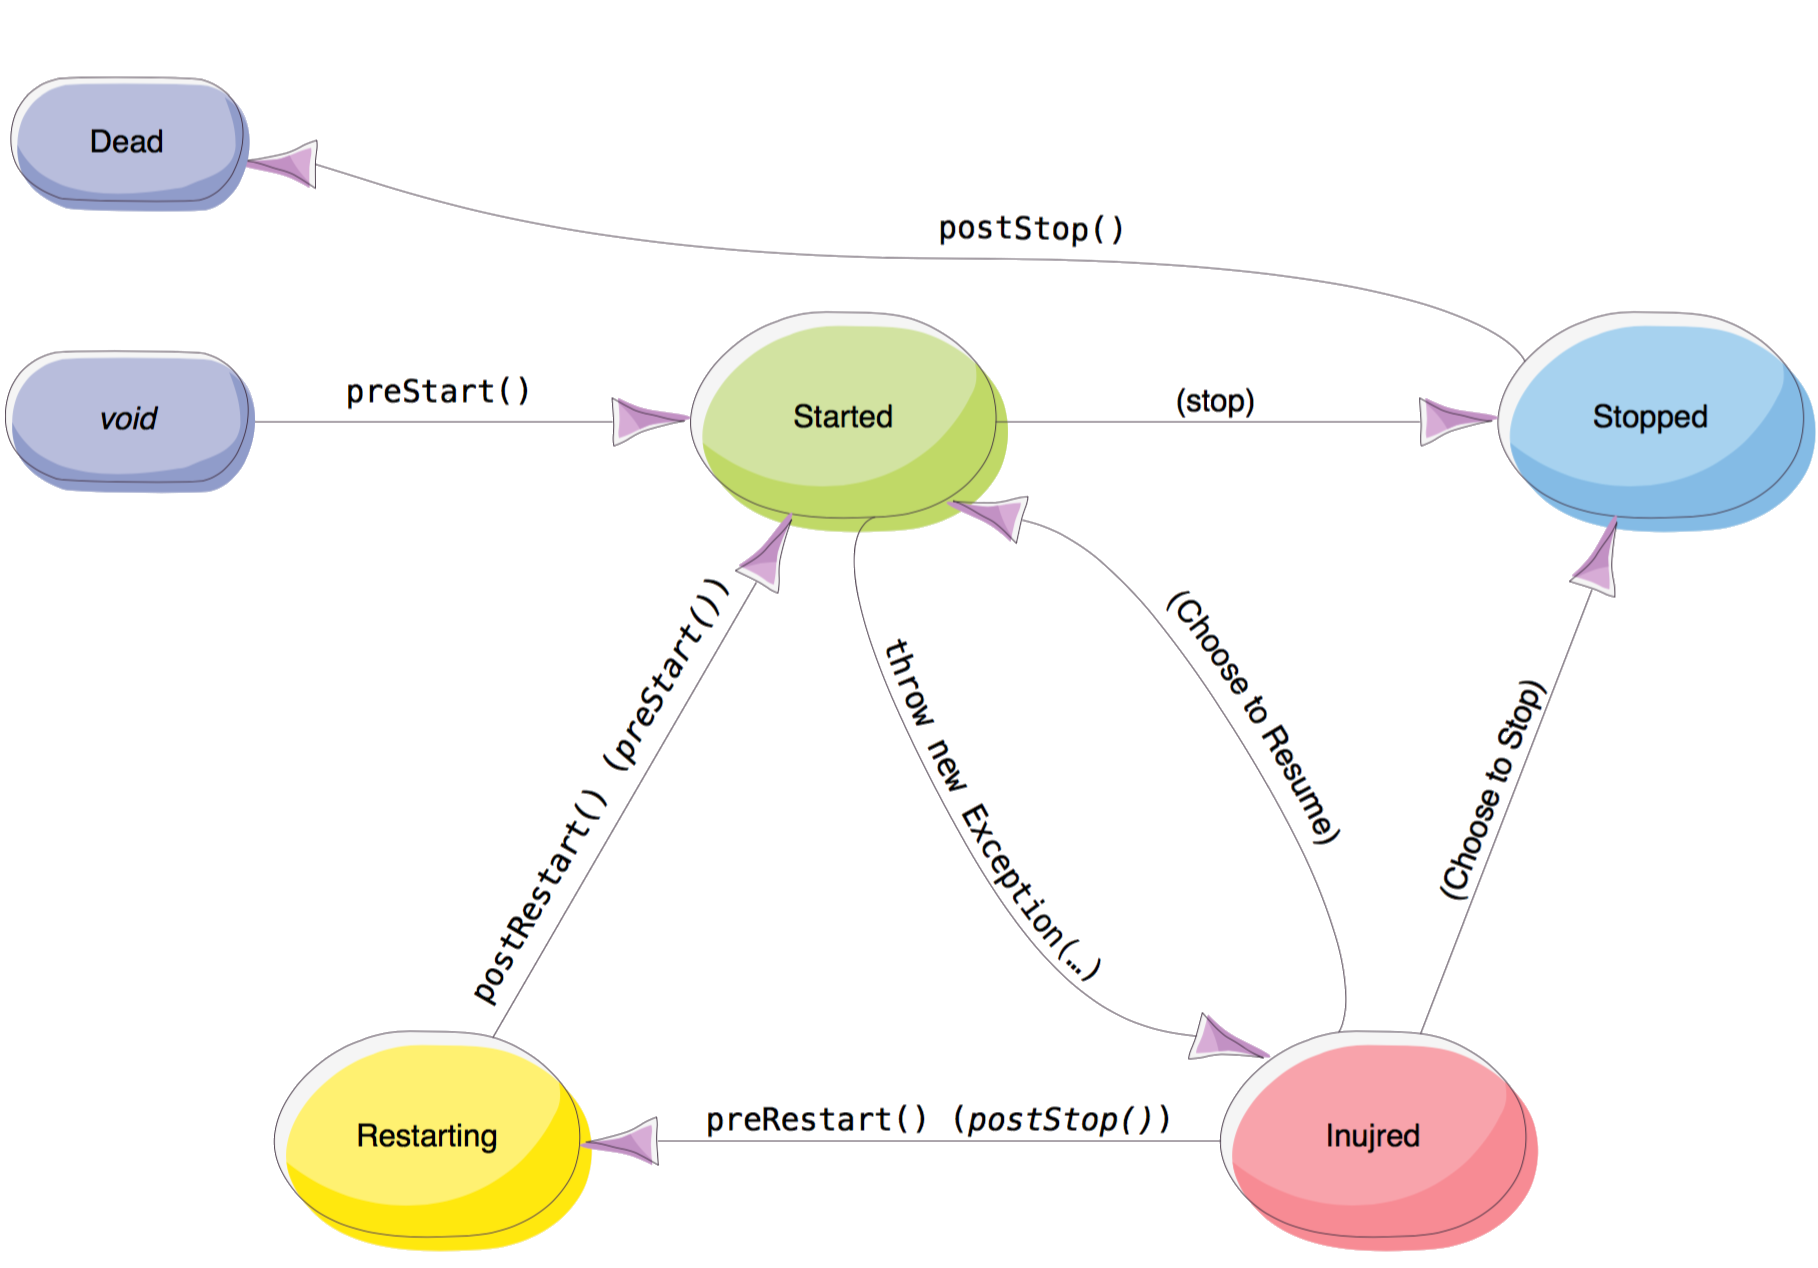
\includegraphics[scale=0.4]{images/analysis/Actor-lifecycle.png}
\caption{Ciclo di vita di un generico attore partecipante al sistema}
\label{analisi-del-problema-distribuzione-recupero-da-fallimento-ciclo-di-vita}
\end{figure}

Attraverso l'utilizzo di tali ``agganci'' è stato possibile conservare e successivamente passare i messaggi ancora nella \english{mailbox} alla nuova istanza dell'attore, nel caso in cui si fosse deciso di riavviarlo; oppure informare altri attori dell'avvenuto errore cosicché potessero attivare una procedura per il recupero del riferimento alla nuova istanza per poter continuare la simulazione.